\chapter{Comparison of Existing Recommender Systems}

\section{Objective components}

We take a composable approach to collaborative filtering (CF) systems
where a (social) CF minimization 
objective $\mathit{Obj}$ is composed of sums of one or more
objective components:
\begin{align}
\mathit{Obj} = \sum_i \lambda_i \mathit{Obj}_i
\end{align}
Because each objective may be weighted differently, a 
weighting term $\lambda_i \in \R$ is included for each component and should be
optimized via cross-validation.

%{\it Binary and ternary prediction:} 
Most target predictions are binary 
classification-based ($\{0,1\}$), therefore
in the objectives a sigmoidal transform 
\begin{align}
\sigma(o) & = \frac{1}{1 + e^{-o}}
\end{align}
of regressor outputs $o \in \R$ is used to squash it 
to the range $[0, 1]$.  
In places where the $\sigma$ transform may be optionally included, 
this is written as $[\sigma]$.  

\begin{comment}
\subsection{Probabilistic Matrix Factorization}


Probabilistic Matrix Factorization tries to model the user preference matrix as a product of 2 lower-rank user and item matrices. The predicted rating of user $i$ on movie $j$ is $U_i^TV_j$. Additionally, $\lambda$ is the regularization parameter and $I_{ij}$ is an indicator function that is equal to 1 if user $i$ rated movie $j$ and equal to 0 otherwise. PMF minimizes the following error function:

\[
E = \frac{1}{2} \sum_{i=1}^N \sum_{j=1}^M \mathbf I_{ij} {(\mathbf R_{ij}-\mathbf U_i^T \mathbf V_j)^2} 
+ \frac{\lambda}{2} \sum _{i=1}^N ||\mathbf U_i||^2_{Fro}
+ \frac{\lambda}{2} \sum _{j=1}^M ||\mathbf V_j||^2_{Fro}
\]


\begin{align}
\sum_{(\x,\y) \in D} \frac{1}{2} (R_{\x,\y} - [\sigma] U^T V)^2
\end{align}
\end{comment}

\subsection{Matchbox Matrix Factorization}

The basic objective function we use for our MF models is the Matchbox~\cite{matchbox} model. Matchbox extends the matrix factorization model~\cite{pmf}  for CF by using the user features and item features in learning the latent spaces for these users and items. The Matchbox MF objective component is:

\begin{align}
\sum_{(\x,\y) \in D} \frac{1}{2} (R_{\x,\y} - [\sigma] \x^T U^T V y)^2
\end{align}

\begin{comment}
One weakness of PMF is that it has a hard time making predictions for users that have made very few or no ratings, and for movies that have been given few or no ratings. To fix this, we can incorporate the user and movie features into the matrix factorization to help bootstrap predictions. Incorporating user and movie features also improve predictions even for users and movies that have had lots of ratings. The objective function of Matchbox Matrix Factorization with Features that is being minimized is
\end{comment}

\begin{comment}
\[
E = \frac{1}{2} \sum_{i=1}^N \sum_{j=1}^M \mathbf I_{ij} {(\mathbf R_{ij}-\mathbf{s}^T \mathbf{t})^2} 
+ \frac{\lambda}{2} ||\mathbf U_i||^2_{Fro}
+ \frac{\lambda}{2} ||\mathbf V_j||^2_{Fro}
\]
\end{comment}

\subsection{L2 Regularization}

To help in generalization, it is important to regularize the free parameters $U$ and $V$ to prevent overfitting in
the presence of sparse data. This can be done with the
$L_2$ regularizer that models a prior of $0$ on the parameters. The objective components for the L2 regularizers are

\begin{align}
\frac{1}{2} \| U \|_\Fro^2 = \frac{1}{2} \tr(U^T U)
\end{align}

\begin{align}
\frac{1}{2} \| V \|_\Fro^2 = \frac{1}{2} \tr(V^T V)
\end{align}

\subsection{Social Regularization}
\label{sec:SocRec}
The social aspect of SCF is implemented as a regularizer on the user matrix $U$. What this objective component does is constrain users with a high similarity rating to have the same values in the latent feature space. This models the assumption that users who are similar socially should also have similar preferences for items.
\\

This method is an extension of existing SCF techniques~\cite{lla,socinf} that constrain the latent space to enforce users  to have similar preferences latent representations when they interact heavily. Like Matchbox which extends regular matrix factorization methods by making use of user and link features, our extension to the Social Regularization method incorporates user features to learn similarities between users in the latent space.

\begin{align}
\sum_{\x} & \sum_{\z \in \mathit{friends}(\x)} \frac{1}{2} (S_{\x,\z} - \la U\x, U\z \ra)^2 \nonumber \\
& = \sum_{\x} \sum_{\z \in \mathit{friends}(\x)} \frac{1}{2} (S_{\x,\z} - \x^T U^T U \z)^2
\end{align}

\subsection{Derivatives}

We seek to optimize sums of the above objectives and will use
gradient descent for this purpose.  

For the overall objective, the partial derivative 
w.r.t. parameters $\a$ are as follows:
\begin{align*}
\frac{\partial}{\partial \a} \mathit{Obj} & = \frac{\partial}{\partial \a} \sum_i \lambda_i \mathit{Obj}_i\\
& = \sum_i \lambda_i \frac{\partial}{\partial \a} \mathit{Obj}_i \label{eq:sum_der}
\end{align*}

Previously we noted that that we may want to transform
some of the regressor outputs $o[\cdot]$ using $\sigma(o[\cdot])$.  
This is convenient for our partial derivatives as
\begin{align}
 \frac{\partial}{\partial \a}\sigma(o[\cdot]) & = \sigma(o[\cdot]) (1 - \sigma(o[\cdot])) \frac{\partial}{\partial \a} o[\cdot] .
\end{align}
Hence anytime a $[\sigma(o[\cdot])]$ is optionally 
introduced in place of $o[\cdot]$, we simply
insert $[\sigma(o[\cdot]) (1 - \sigma(o[\cdot]))]$ in the corresponding derivatives 
below.\footnote{We note that our experiments using the sigmoidal transform in
objectives with $[0,1]$ predictions do not generally demonstrate a
clear advantage vs. the omission of this transform as originally
written (although they do not demonstrate a clear disadvantage
either).}

Before we proceed to our objective gradients, we define abbreviations
for two useful vectors:
\begin{align*}
\s & = U \x \qquad \s_{k} = (U \x)_{k}; \; k=1\ldots K\\
\t & = V \y \qquad \t_{k} = (V \y)_{k}; \; k=1\ldots K
\end{align*}

Now we proceed to derivatives for the previously defined primary
objective components:
\begin{itemize}
\item {\bf Matchbox Matrix Factorization}:
Here we define alternating partial derivatives between $U$ and $V$, holding one
constant and taking the derivative w.r.t.\ the other:\footnote{We will use
this method of alternation for all objective components that involve bilinear
terms.}
\begin{align*}
\frac{\partial}{\partial U} \Obj_\pmcf & = \frac{\partial}{\partial U} \sum_{(\x,\y) \in D} \frac{1}{2} \left( \underbrace{(R_{\x,\y} - [\sigma] \overbrace{x^T U^T V\y}^{o_{\x,\y}})}_{\delta_{\x,\y}} \right)^2\\
& = \sum_{(\x,\y) \in D} \delta_{\x,\y} \frac{\partial}{\partial U} - [\sigma] \x^T U^T \t \\
& = - \sum_{(\x,\y) \in D} \delta_{\x,\y} [\sigma(o_{\x,\y}) (1 - \sigma(o_{\x,\y}))] \t \x^T \\
\frac{\partial}{\partial V} \Obj_\pmcf & = \frac{\partial}{\partial V} \sum_{(\x,\y) \in D} \frac{1}{2} \left( \underbrace{(R_{\x,\y} - [\sigma] \overbrace{x^T U^T V\y}^{o_{\x,\y}})}_{\delta_{\x,\y}} \right)^2\\
& = \sum_{(\x,\y) \in D} \delta_{\x,\y} \frac{\partial}{\partial V} - [\sigma] \s^T V \y \\
& = - \sum_{(\x,\y) \in D} \delta_{\x,\y} [\sigma(o_{\x,\y}) (1 - \sigma(o_{\x,\y}))] \s \y^T
\end{align*}
\end{itemize}

For the regularization objective components, the derivatives are:

\begin{itemize}
\item {\bf $L_2$ $U$ regularization}:
\begin{align*}
\frac{\partial}{\partial U} \Obj_\ru & = \frac{\partial}{\partial U} \frac{1}{2} \tr(U^T U) \\
& = U
\end{align*}
\item {\bf $L_2$ $V$ regularization}:
\begin{align*}
\frac{\partial}{\partial V} \Obj_\rv & = \frac{\partial}{\partial V} \frac{1}{2} \tr(V^T V) \\
& = V
\end{align*}
\item {\bf Social regularization}:
\begin{align*}
\frac{\partial}{\partial U} \Obj_\rs & = \frac{\partial}{\partial U} \sum_{\x} \sum_{\z \in \mathit{friends}(\x)} \frac{1}{2} \left( \underbrace{S_{\x,\z} - \x^T U^T U \z}_{\delta_{\x,\y}} \right)^2 \\
& = \sum_{\x} \sum_{\z \in \mathit{friends}(\x)} \delta_{\x,\y} \frac{\partial}{\partial U} - \x^T U^T U \z \\
& = - \sum_{\x} \sum_{\z \in \mathit{friends}(\x)} \delta_{\x,\y} U (\x \z^T + \z \x^T)
\end{align*}

\end{itemize}

Hence, for any choice of primary objective and one or more regularizers,
we simply add the derivatives for $U$ and/or $V$ 
according to~\eqref{eq:sum_der}.

% Local Variables: 
% mode: latex
% TeX-master: "thesis"
% End: 


\section{Algorithms}

The CF and SCF algorithms used for the first user trial were:

\begin{enumerate}
\item{ {\bf $k$-Nearest Neighbor}}
\item{{\bf Support Vector Machines}}
\item{{\bf Matchbox}: Matchbox MF  + L2 Regularization}
\item{{\bf Social Matchbox}: Matchbox MF + Social Regularization + L2 Regularization}
\end{enumerate}

Social Matchbox uses the Social Regularization method to incorporate the social information of the FB data. SVM, Matchbox and Nearest Neighbors do not make use of any social information and are collaborative filtering recommenders.

\section{Online Results}

The first live user trial was run from August 1 to October 13, though we include only data starting from August 25 in our results because that is when the parameters of the algorithms were finalized. The algorithms were randomly distributed among the 106 users who installed the LinkR application. The distribution of the algorithms to the users are show in Table~\ref{tab:Assigned1}

Each user was recommended 3 links everyday and they were able to rate the links on whether they `Liked' or `Disliked' it. Results shown are the number of Like ratings and the number of Dislike ratings normalized by the total number of ratings (Likes + Dislikes) per algorithm. 

As shown in Figure~\ref{fig:OnlineResult1}, Social Matchbox was the best performing algorithm in the first trial and in fact was the only algorithm to get receive more like ratings than dislike ratings. This would suggest that using social information does indeed provide useful information that resulted in better link recommendations from LinkR.

\begin{table}[h!]
\centering
\begin{tabular}{| l | c |}
\hline
{\bf Algorithm} & {\bf Users} \\
\hline
Social Matchbox & 26\\
Matchbox  & 26 \\
SVM & 28 \\
Nearest Neighbor & 28 \\
\hline
\end{tabular}
\caption{Number of Users Assigned per Algorithm.}
\label{tab:Assigned1}
\end{table}

\begin{figure}[h!]
\centering
\subfigure{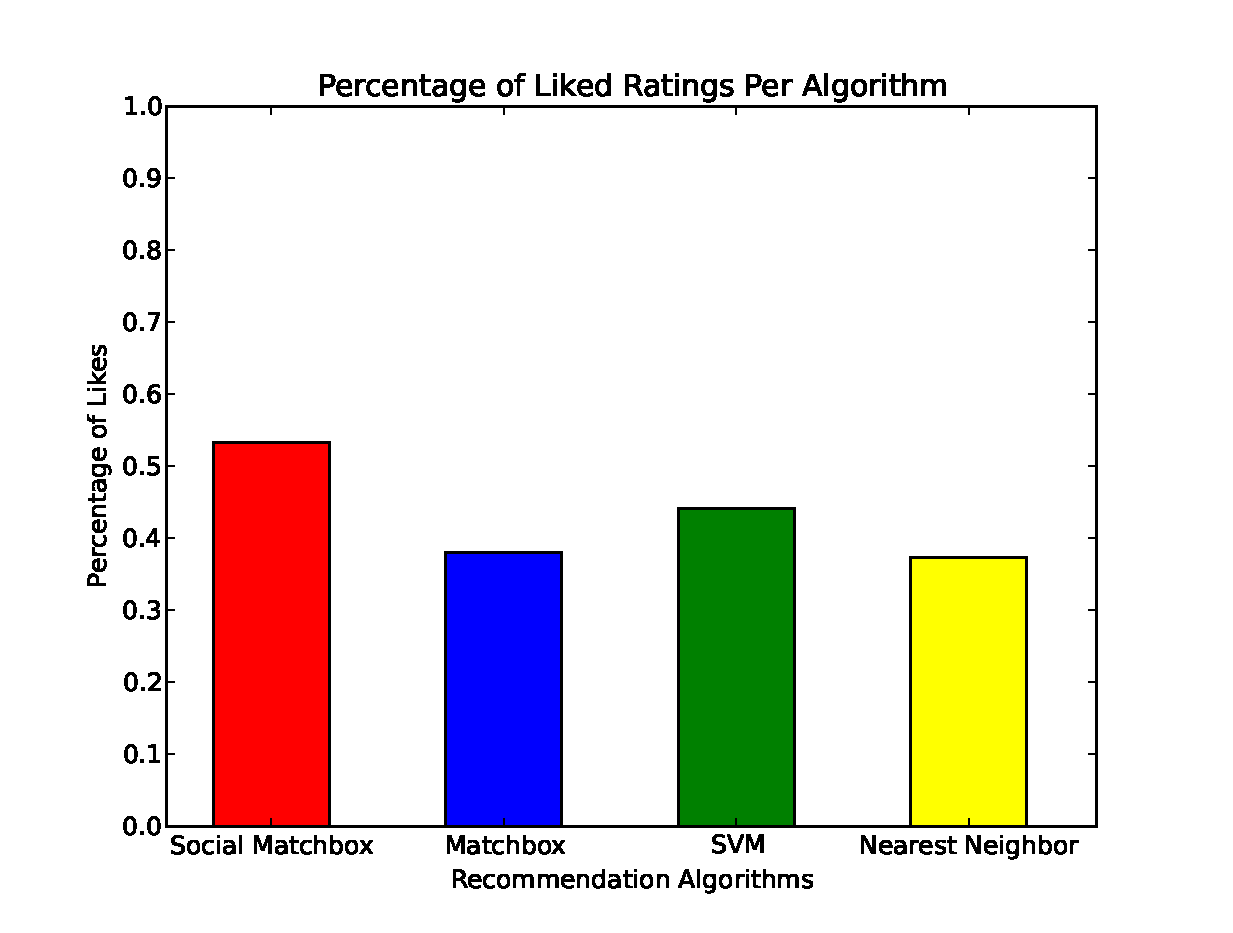
\includegraphics[scale=0.35]{img/live-likes1.eps}}
\subfigure{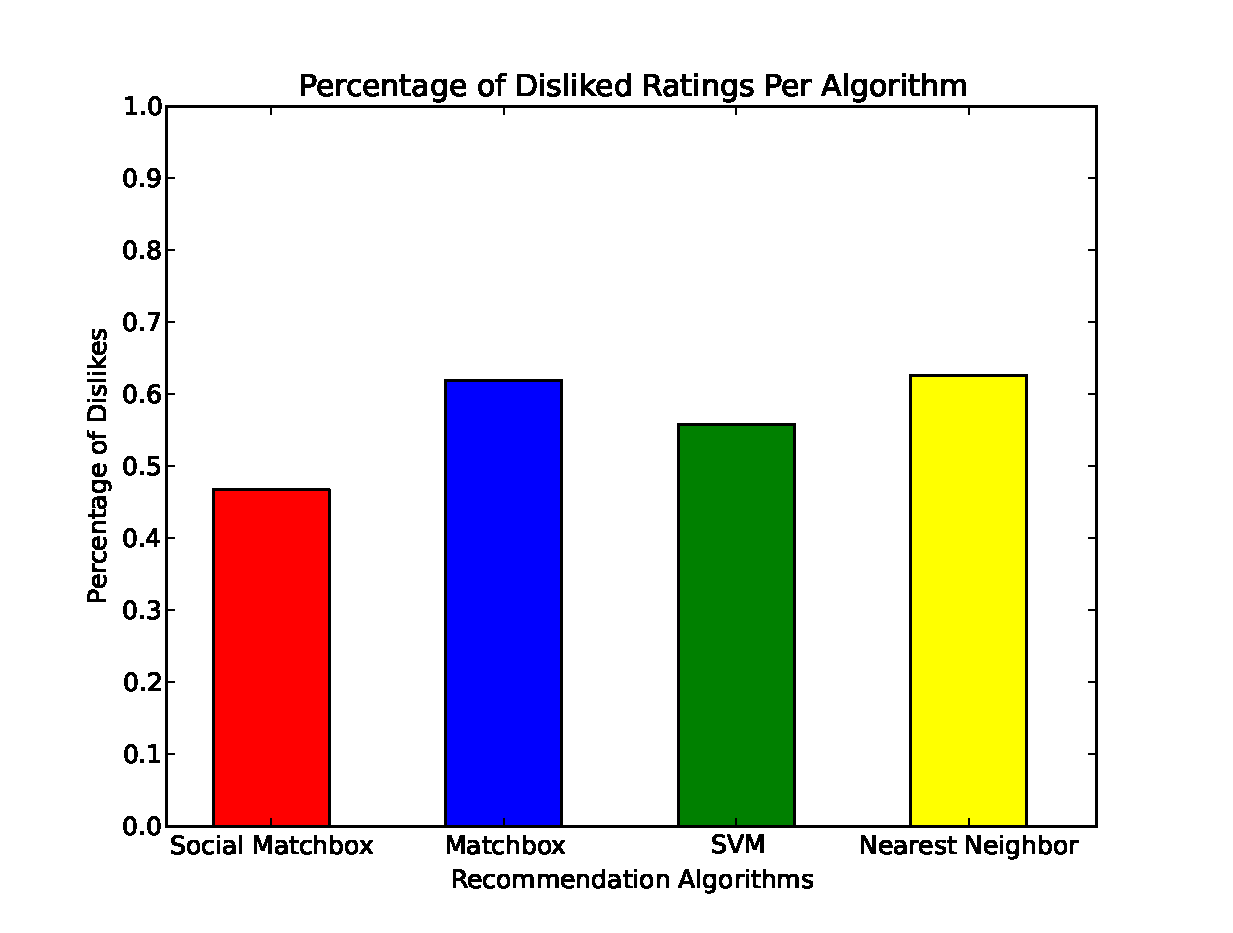
\includegraphics[scale=0.35]{img/live-dislikes1.eps}}
\caption{Results of the online live trials. Social Matchbox was found to be the best performing algorithm.}
\label{fig:OnlineResult1}
\end{figure}

We also look at the algorithms with the results split between friend links and non-friend links recommendations. Again, the results shown are the number of Likes or Dislikes from friends or non-friends normalized by the total number of ratings on those types of recommendations. As shown in Figure~\ref{fig:OnlineFriend1}, all four algorithms experienced a significant performance drop in the ratio of Likes to Dislikes when it came to recommending non-friend links. This suggests that aside from Liking or Disliking a link solely from the quality of the link being recommended, users are also more likely to Like a link simply because a friend had posted it and more likely to Dislike it because it was posted by a stranger.

\begin{figure}[h!]
\centering
\subfigure{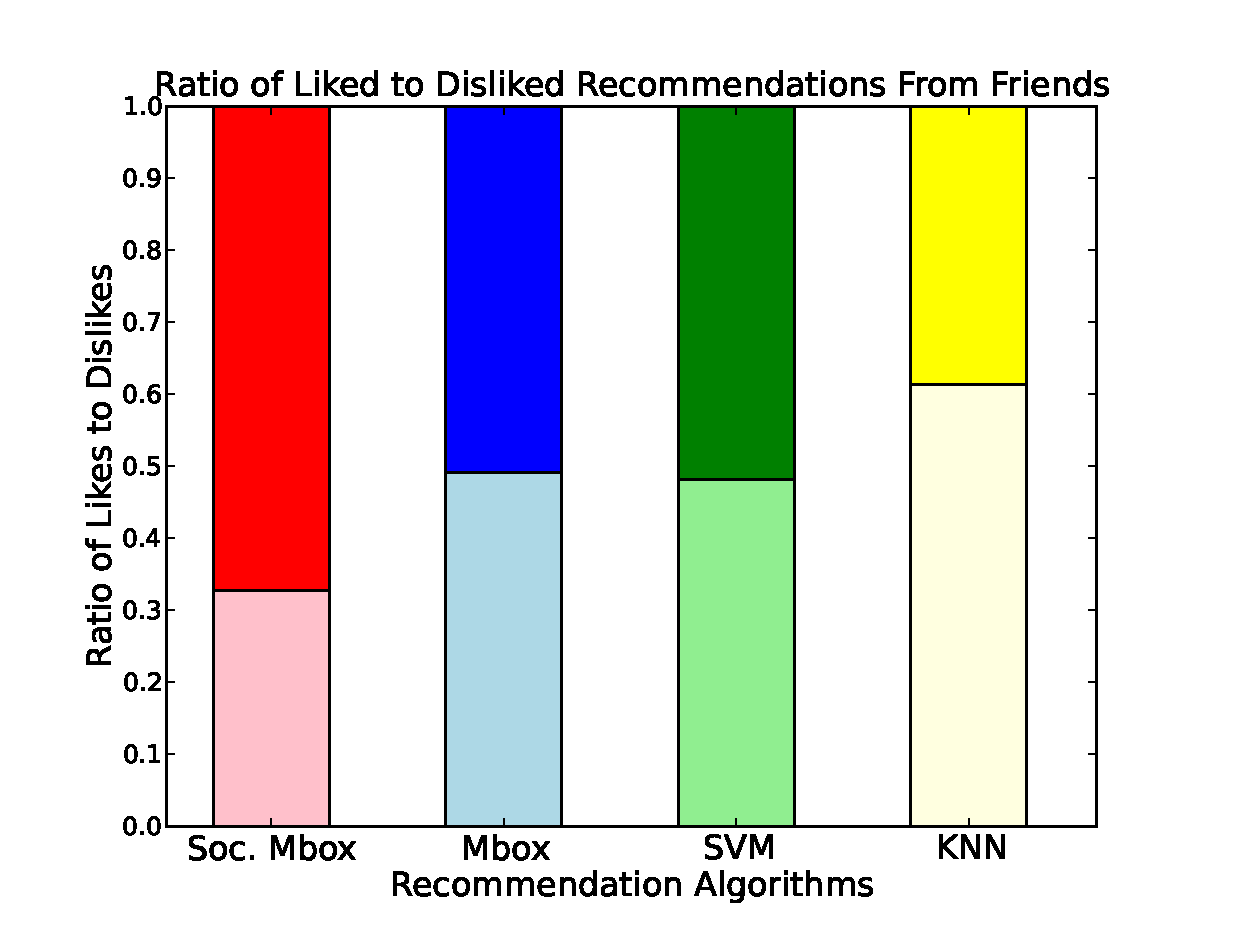
\includegraphics[scale=0.35]{img/live-friend-likes1.eps}}
\subfigure{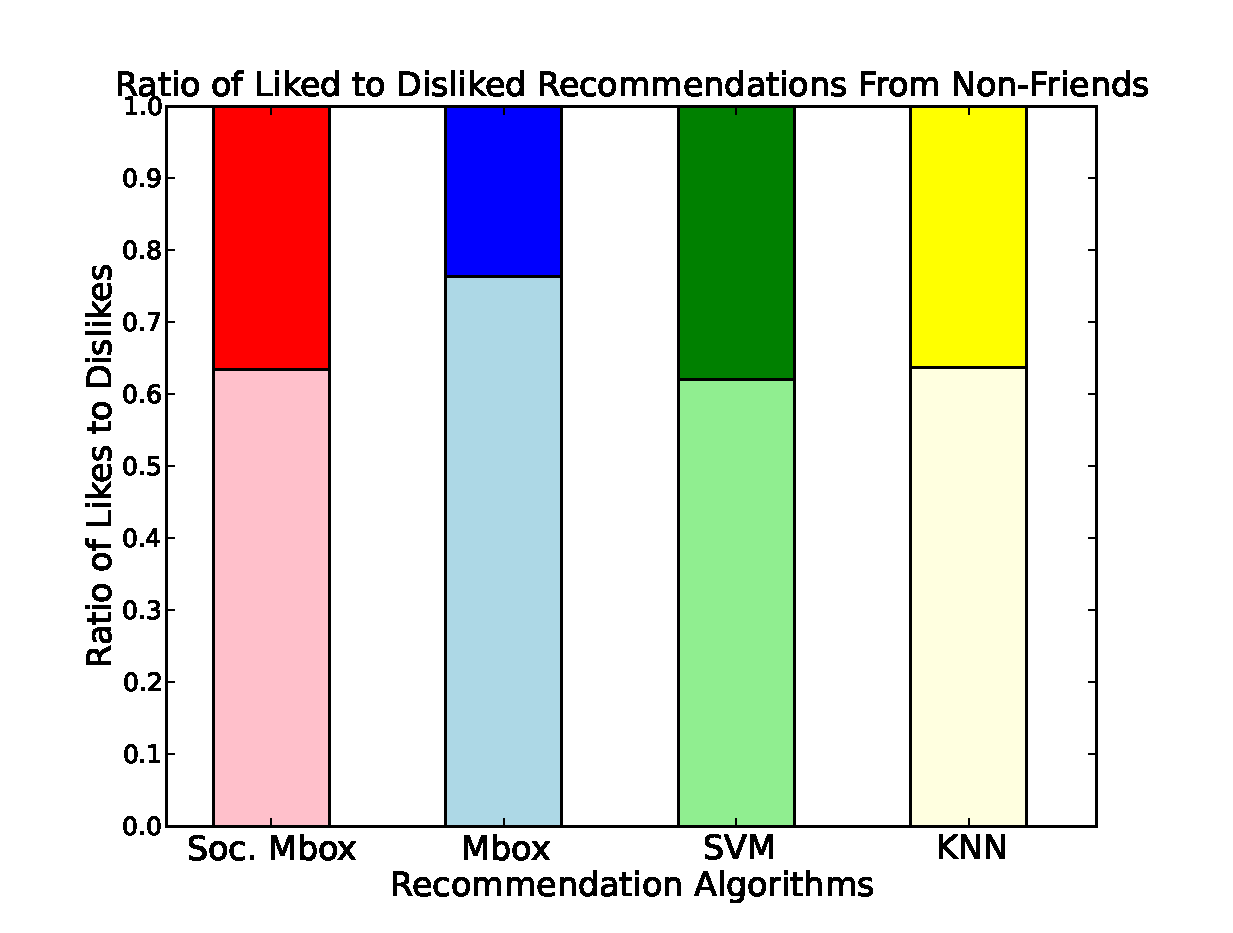
\includegraphics[scale=0.35]{img/live-nonfriend-likes1.eps}}
\subfigure{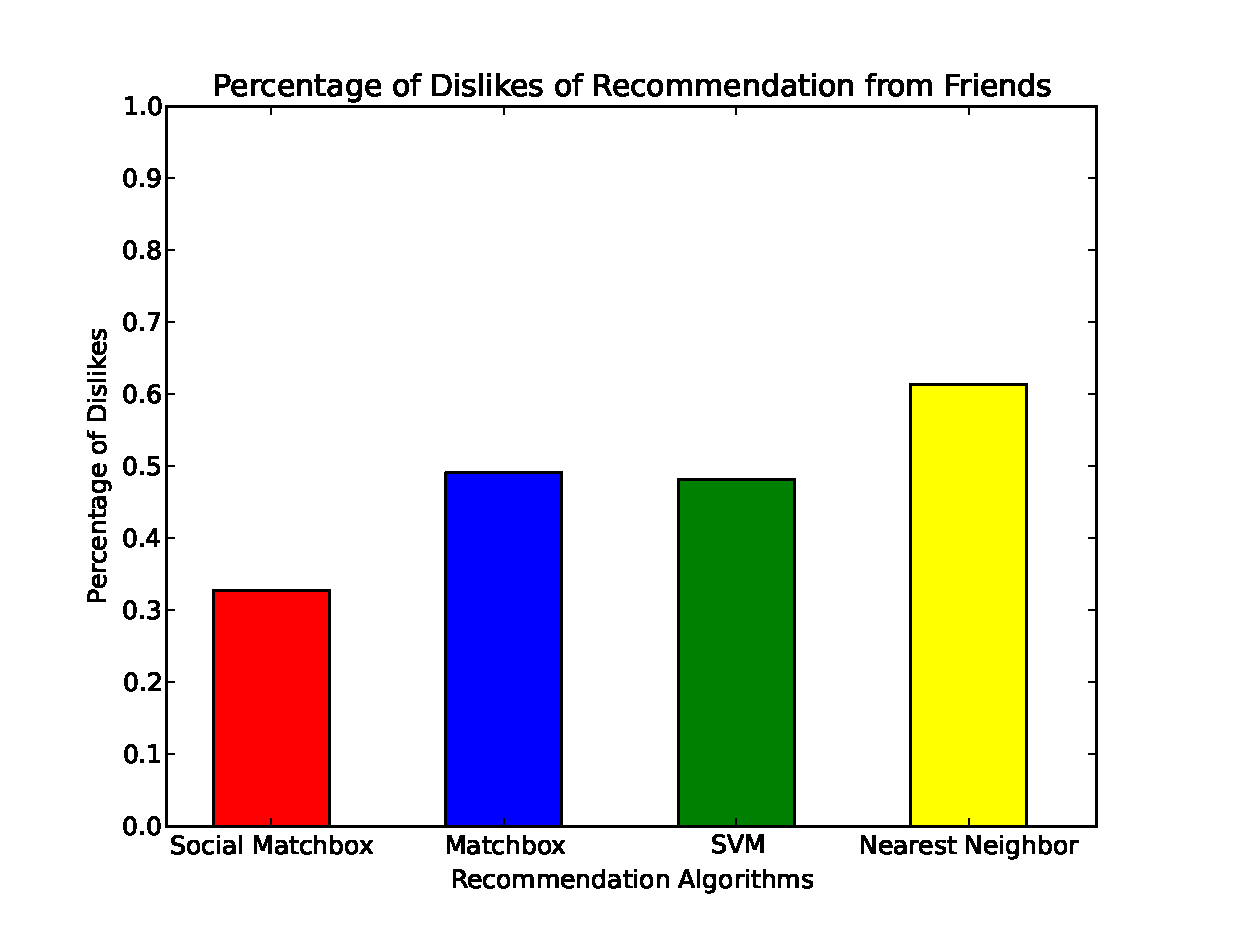
\includegraphics[scale=0.35]{img/live-friend-dislikes1.eps}}
\subfigure{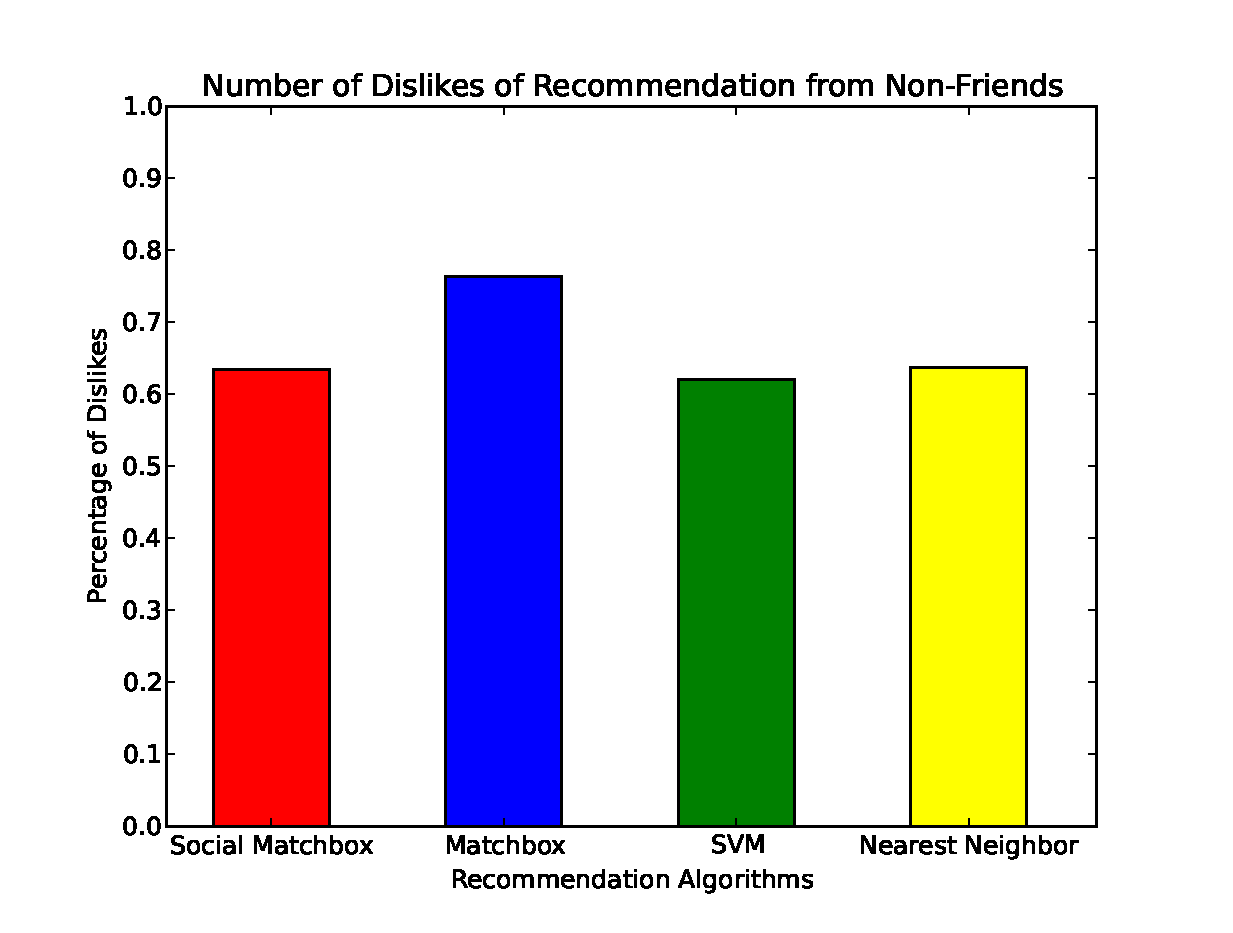
\includegraphics[scale=0.35]{img/live-nonfriend-dislikes1.eps}}
\caption{Results of the online live trials, split between friends and non-friends. There is a significant drop in performance between recommending friend links and recommending non-friend links.}
\label{fig:OnlineFriend1}
\end{figure}

\section {Offline Results}

The goal of the offline experiments was to see how best to reproduce the results of the live experiments offline. As discussed in Chapter 3, the algorithms are being evaluated using the Mean Average Precision metric. The offline experiments were also used to tune the parameters of the different algorithms. 

When training on the UNION dataset, we can find the same general worsening of performance between the results of testing on APP-USER-ACTIVE-FRIENDS and APP-USER-ACTIVE-NON-FRIENDS. Additionally, when testing on the APP-USER-ACTIVE-ALL, the training/test data combination most similar to the online setup, we find that Social Matchbox again slightly beat the other algorithms.

\begin{figure}[h]
\centering
\subfigure{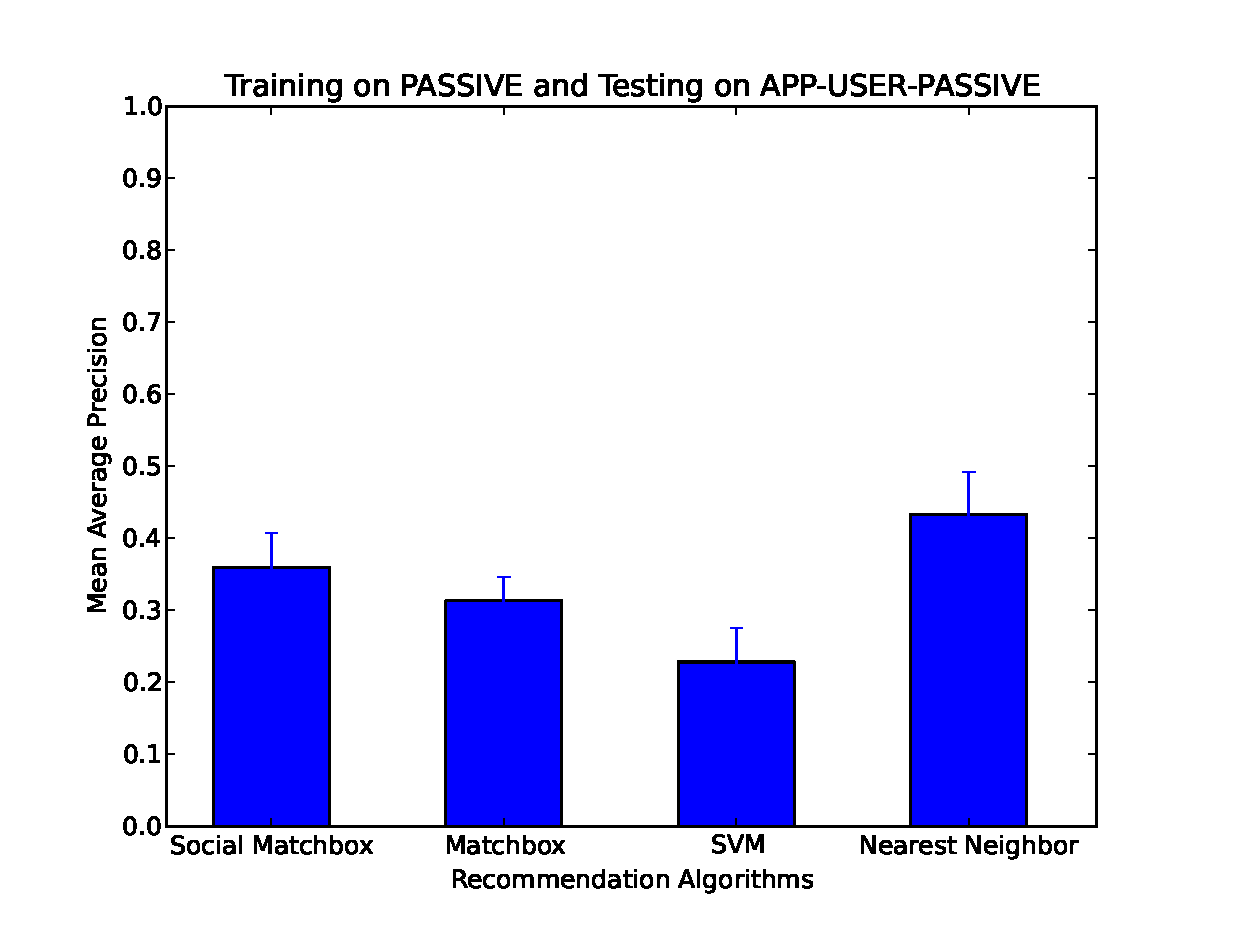
\includegraphics[scale=0.355]{img/Passive_App-User-Passive1.eps}}
\subfigure{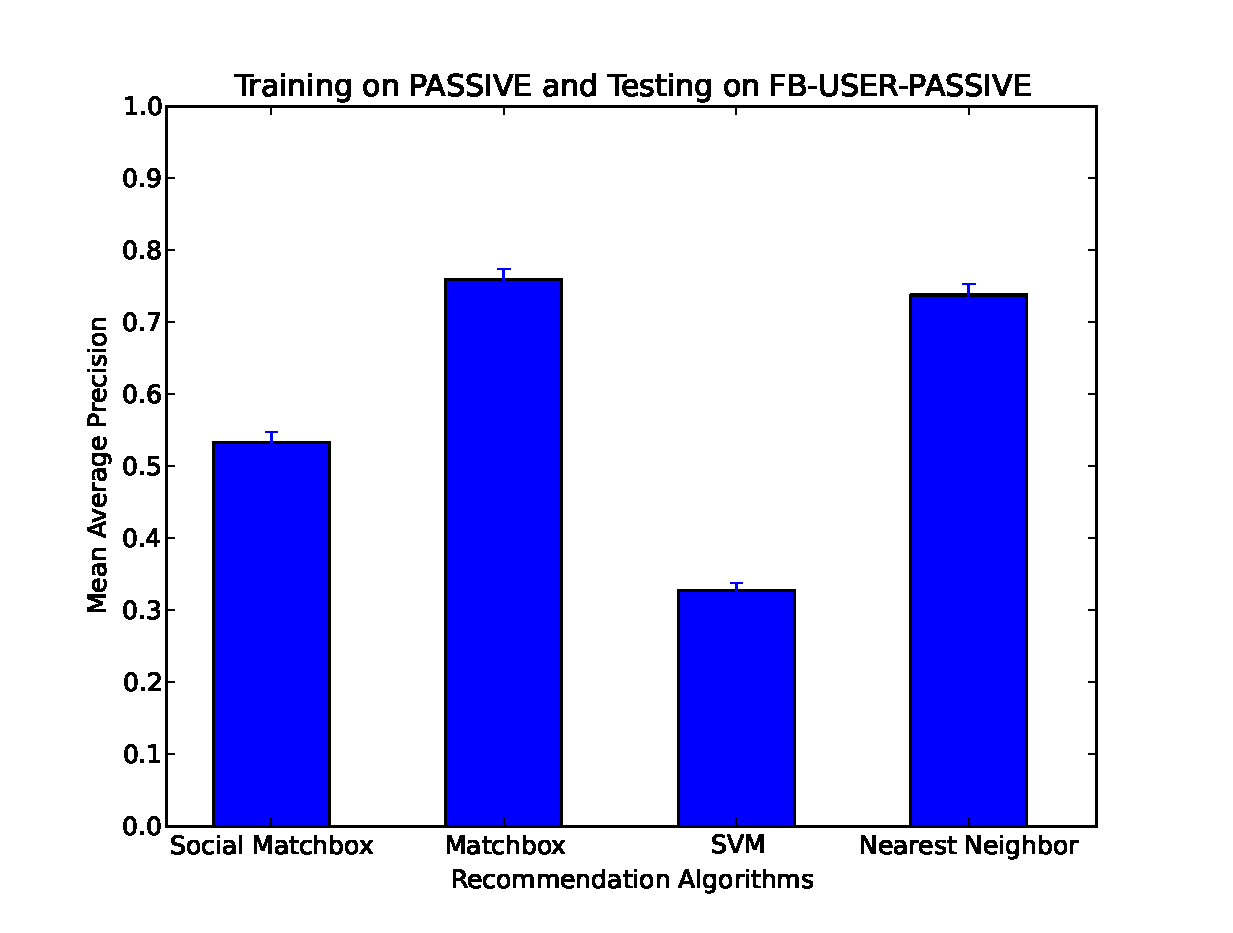
\includegraphics[scale=0.355]{img/Passive_FB-User-Passive1.eps}}
\subfigure{\includegraphics[scale=0.355]{img/Passive_App-User-active-all1.eps}}
\subfigure{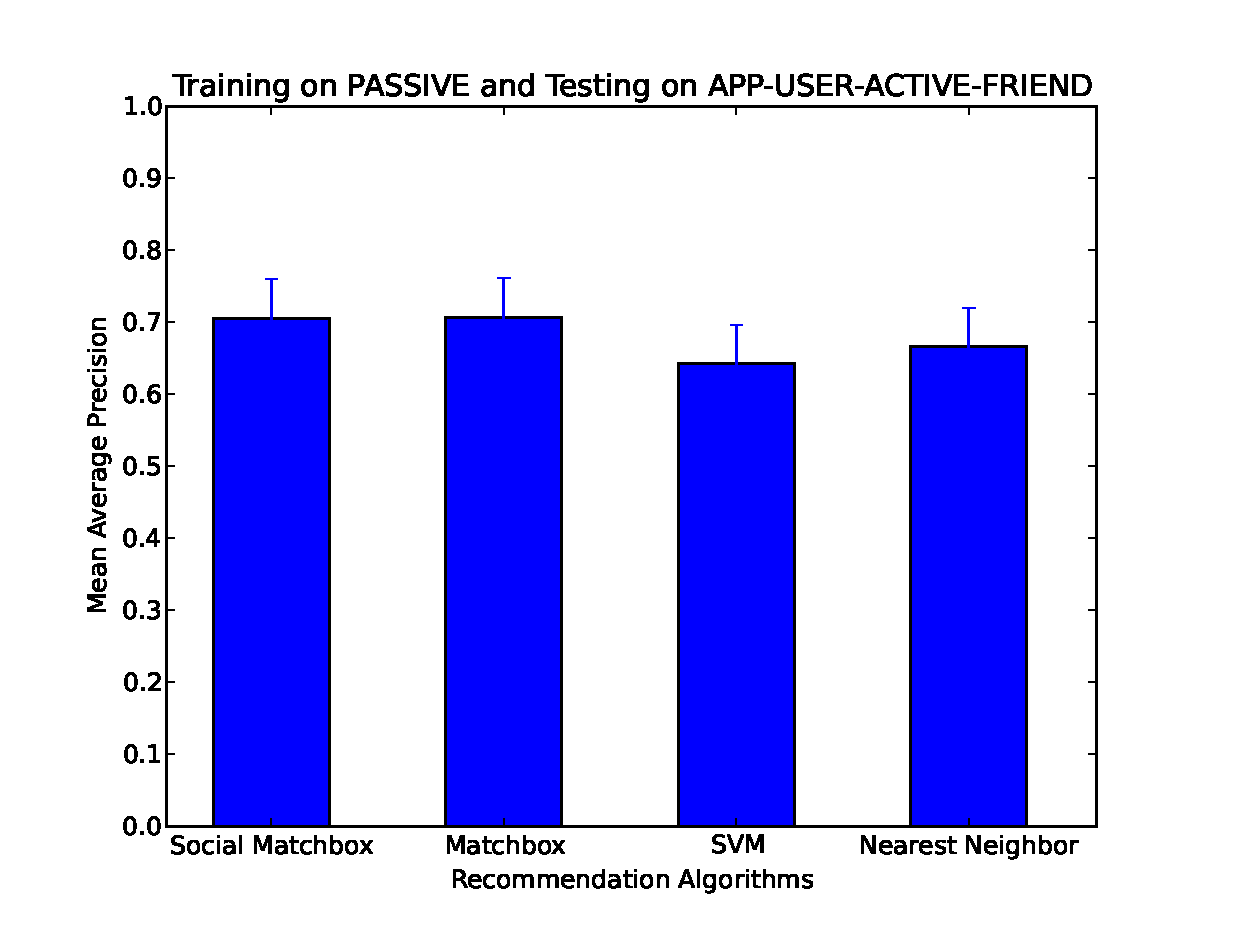
\includegraphics[scale=0.355]{img/Passive_App-User-Active-Friends1.eps}}
\subfigure{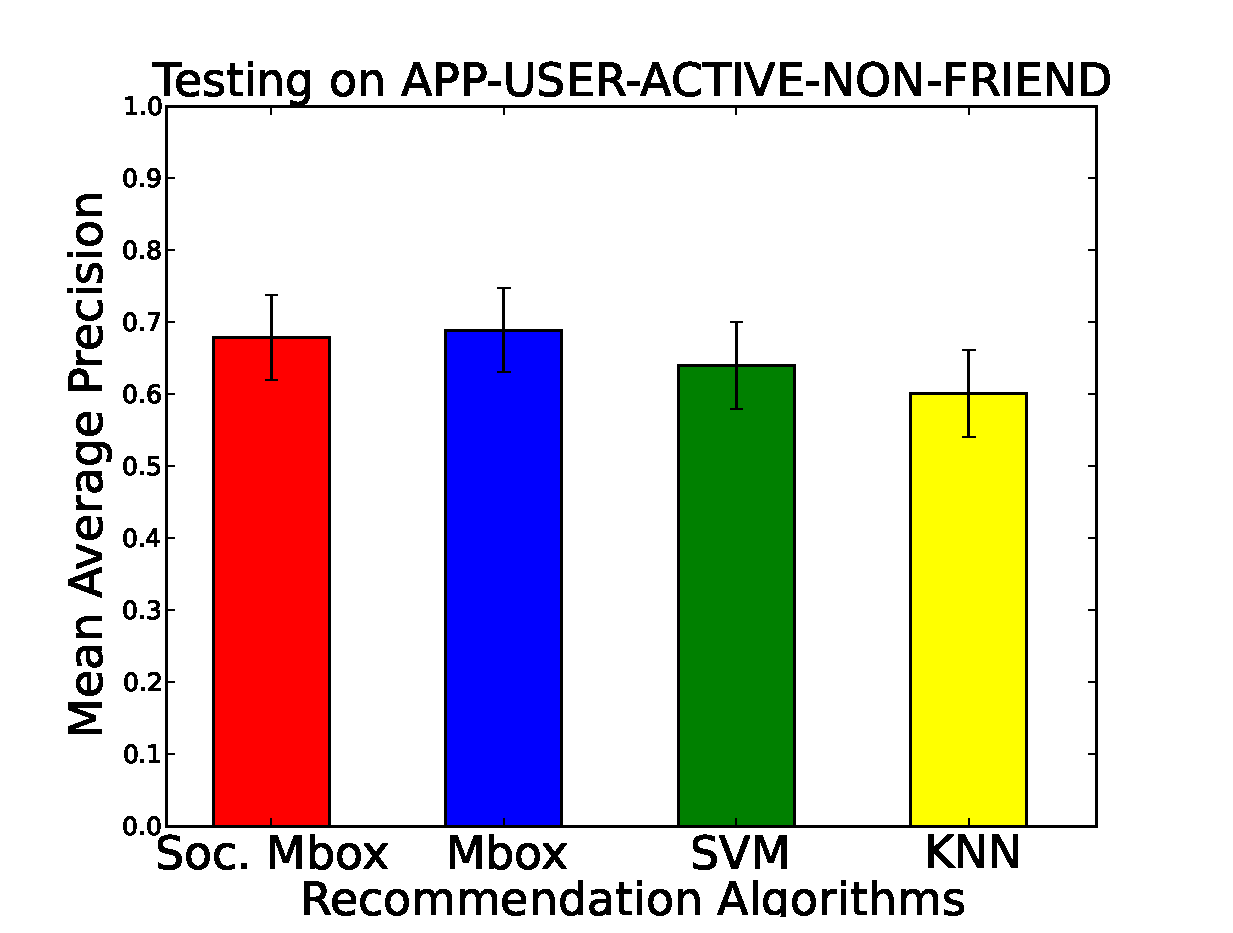
\includegraphics[scale=0.355]{img/Passive_App-User-Active-NonFriends1.eps}}
\caption{Results of training on PASSIVE data}
\end{figure}

\begin{figure}[h]
\centering
\subfigure{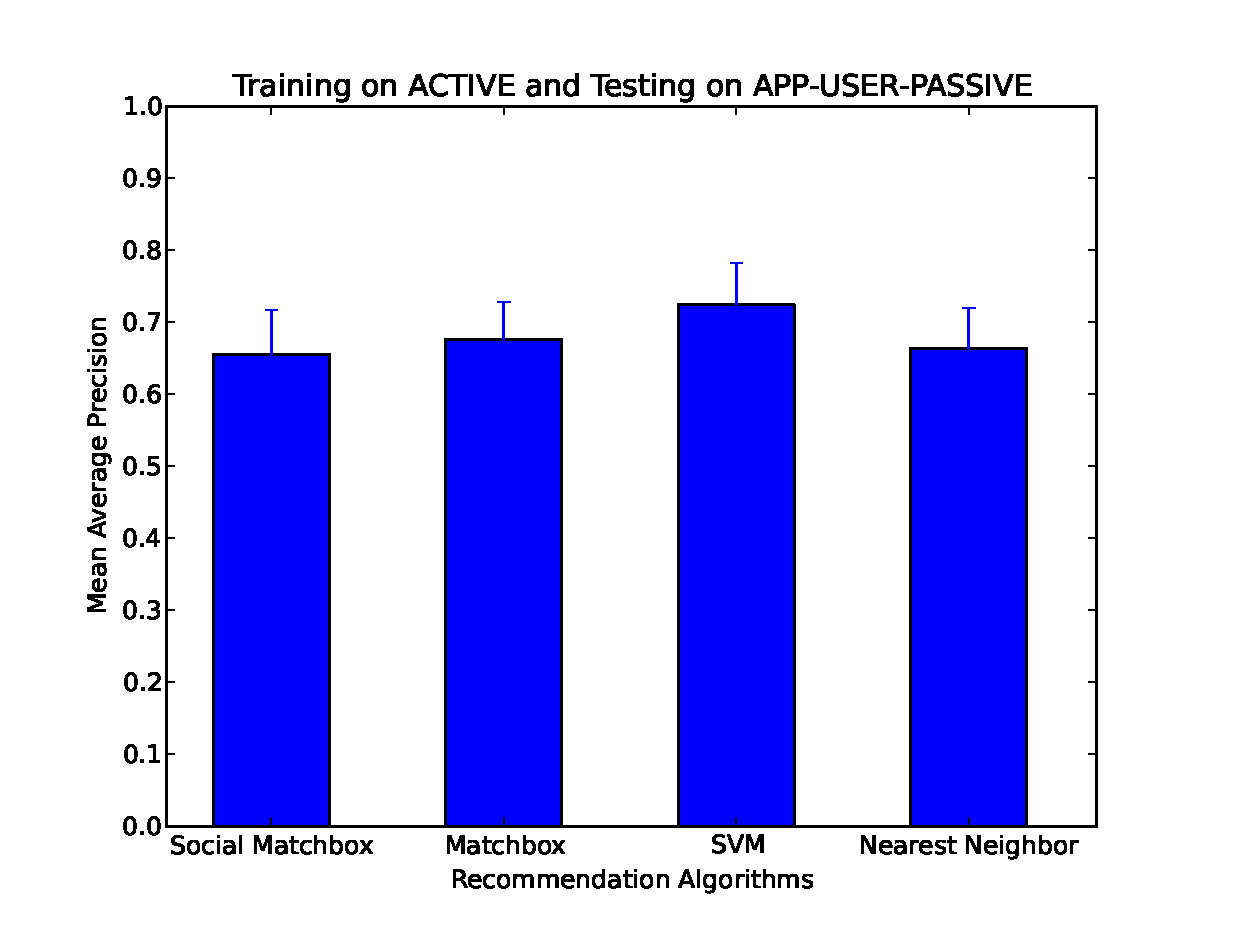
\includegraphics[scale=0.35]{img/Active_App-User-Passive1.eps}}
\subfigure{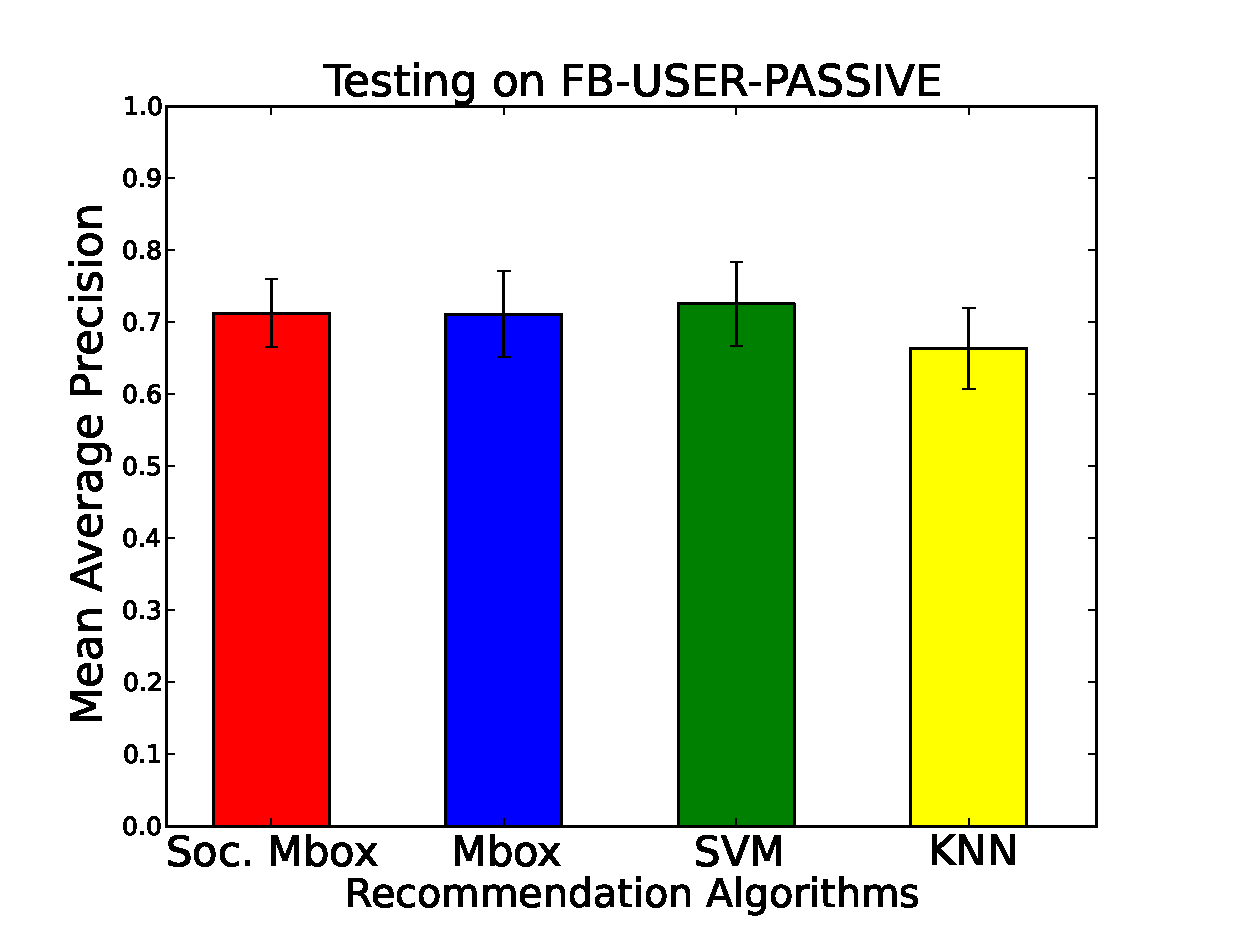
\includegraphics[scale=0.35]{img/Active_FB-User-Passive1.eps}}
\subfigure{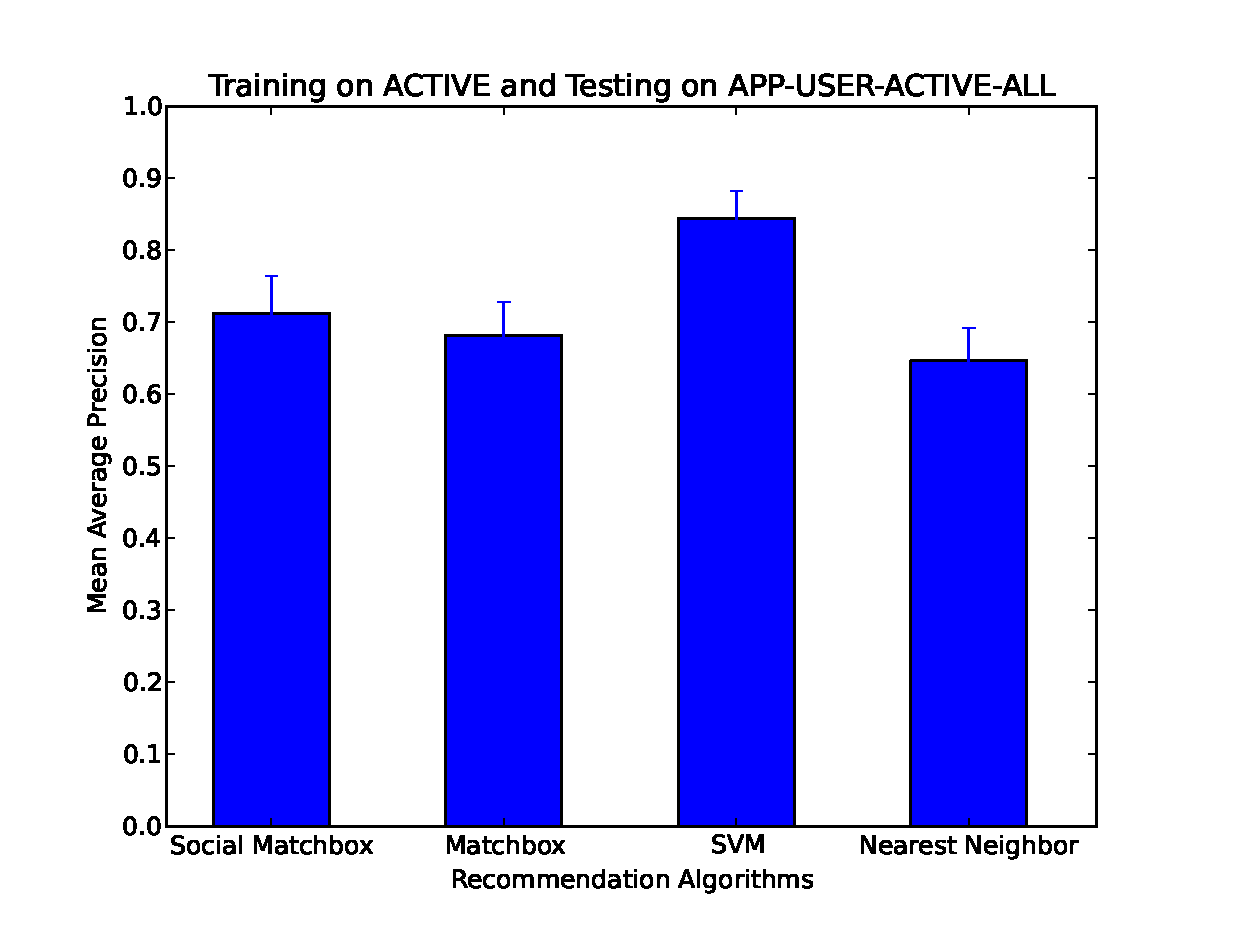
\includegraphics[scale=0.35]{img/Active_App-User-Active-All1.eps}}
\subfigure{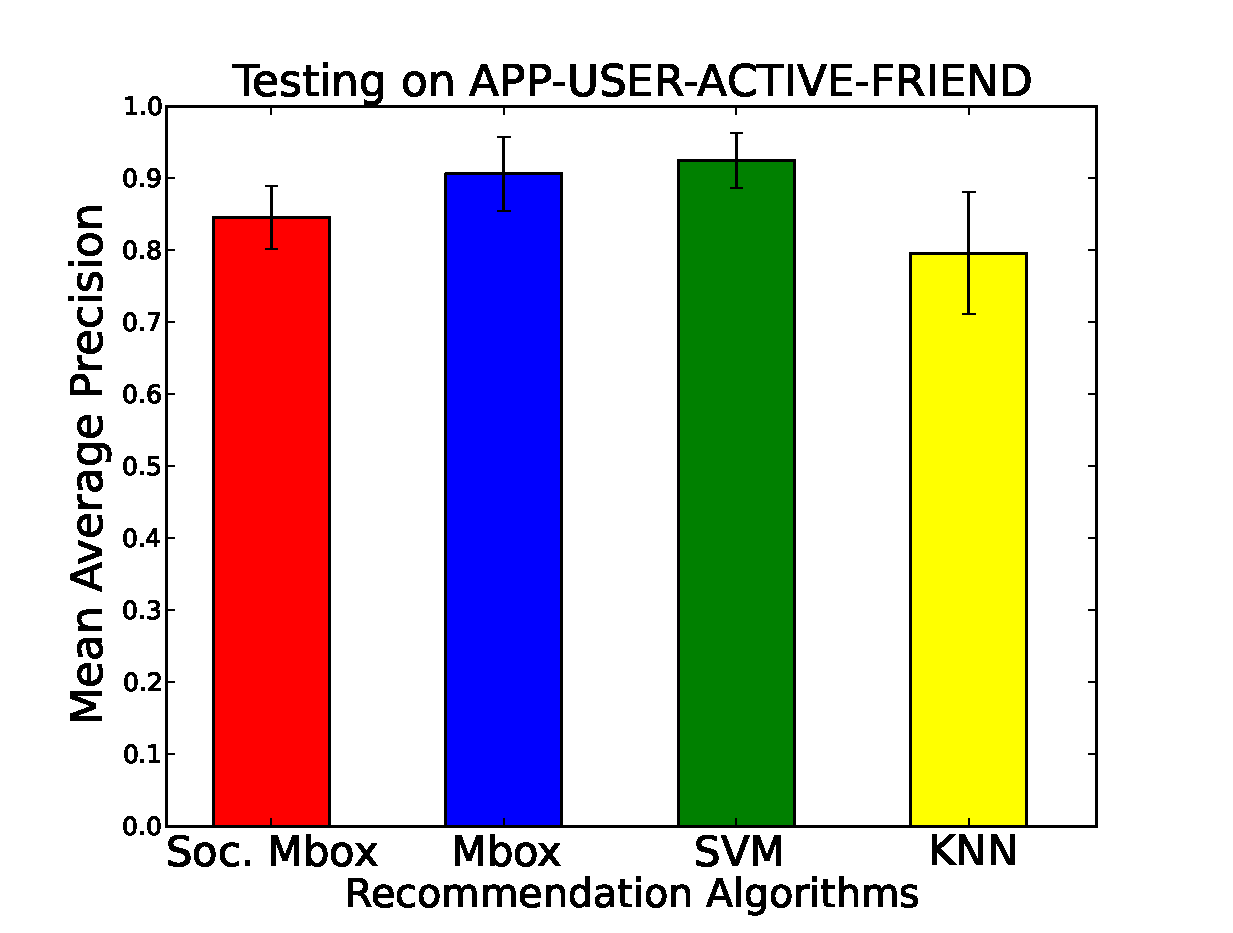
\includegraphics[scale=0.35]{img/Active_App-User-Active-Friends1.eps}}
\subfigure{\includegraphics[scale=0.35]{img/Active_App-User-Active-Nonfriends1.eps}}
\caption{Results of training on ACTIVE data}
\end{figure}

\begin{figure}[h]
\centering
\subfigure{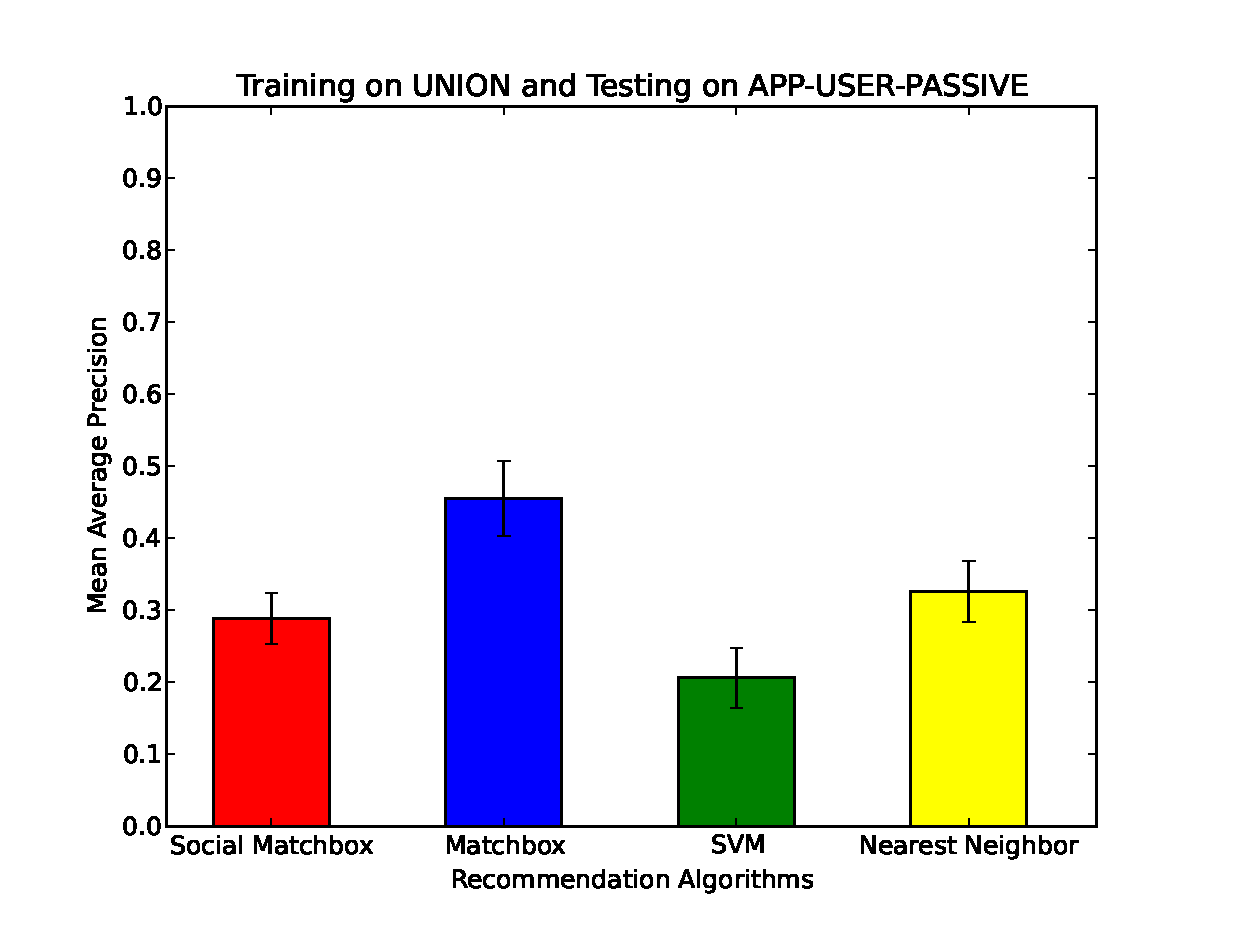
\includegraphics[scale=0.35]{img/Union_App-User-Passive1.eps}}
\subfigure{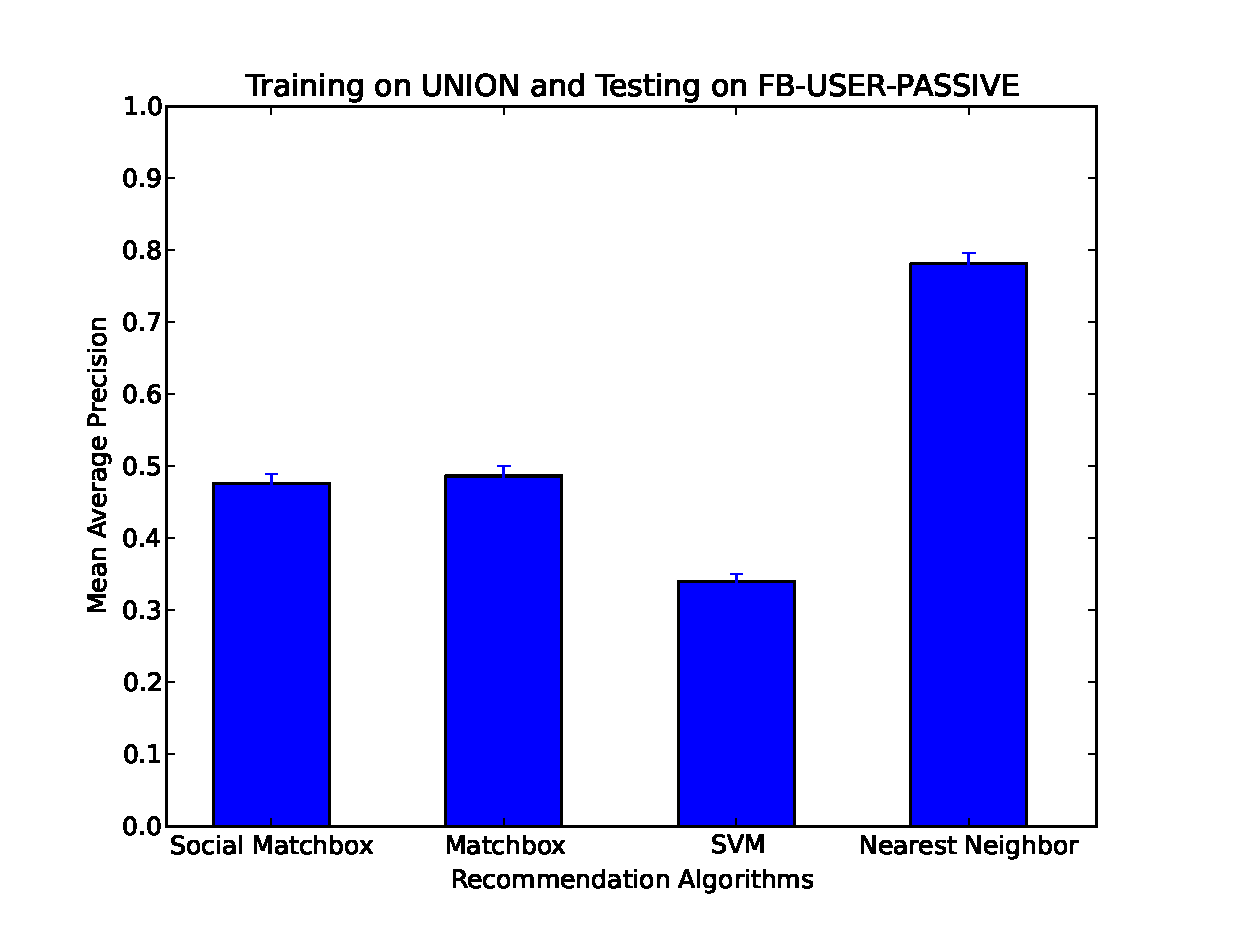
\includegraphics[scale=0.35]{img/Union_FB-User-Passive1.eps}}
\subfigure{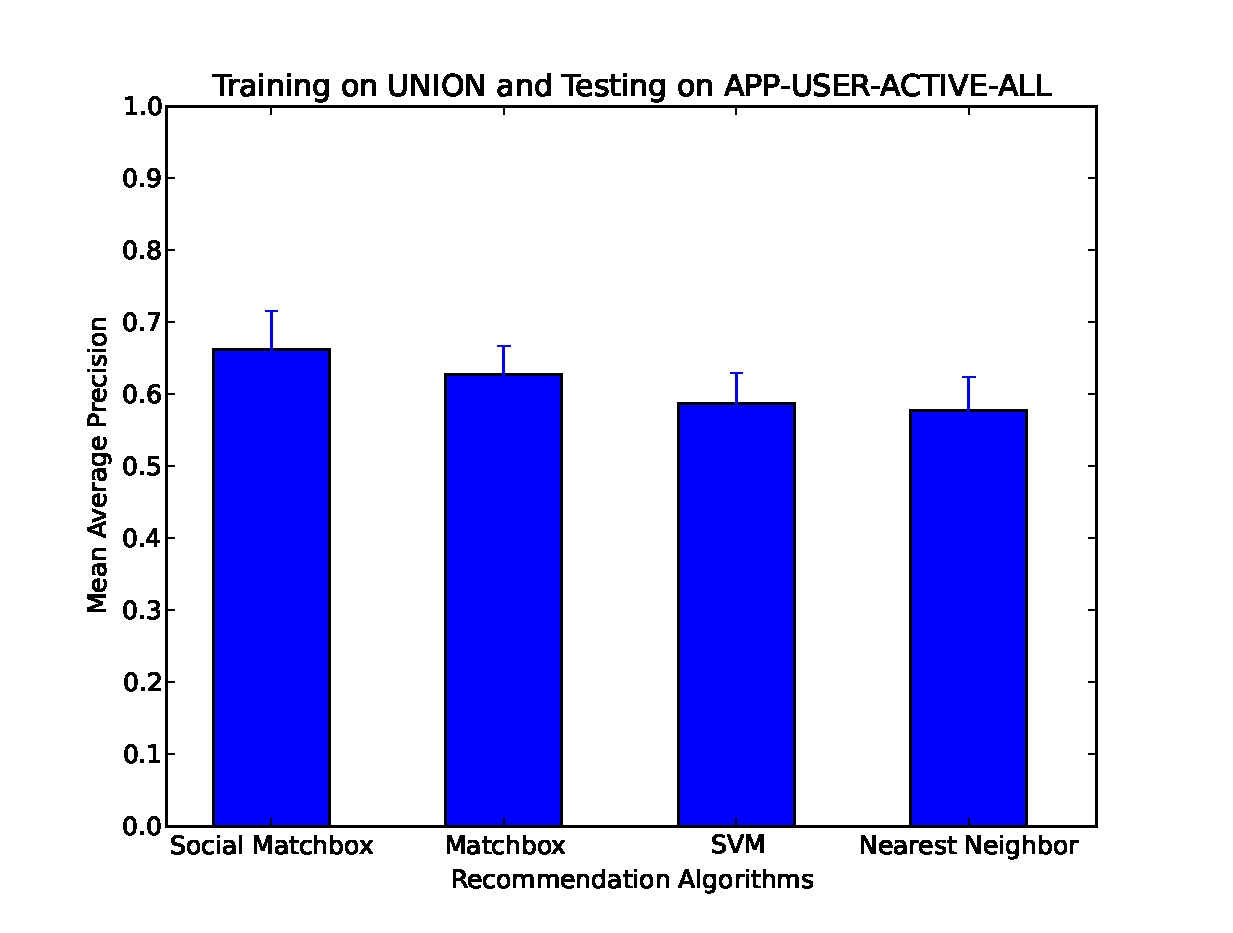
\includegraphics[scale=0.35]{img/Union_App-User-Active-All1.eps}}
\subfigure{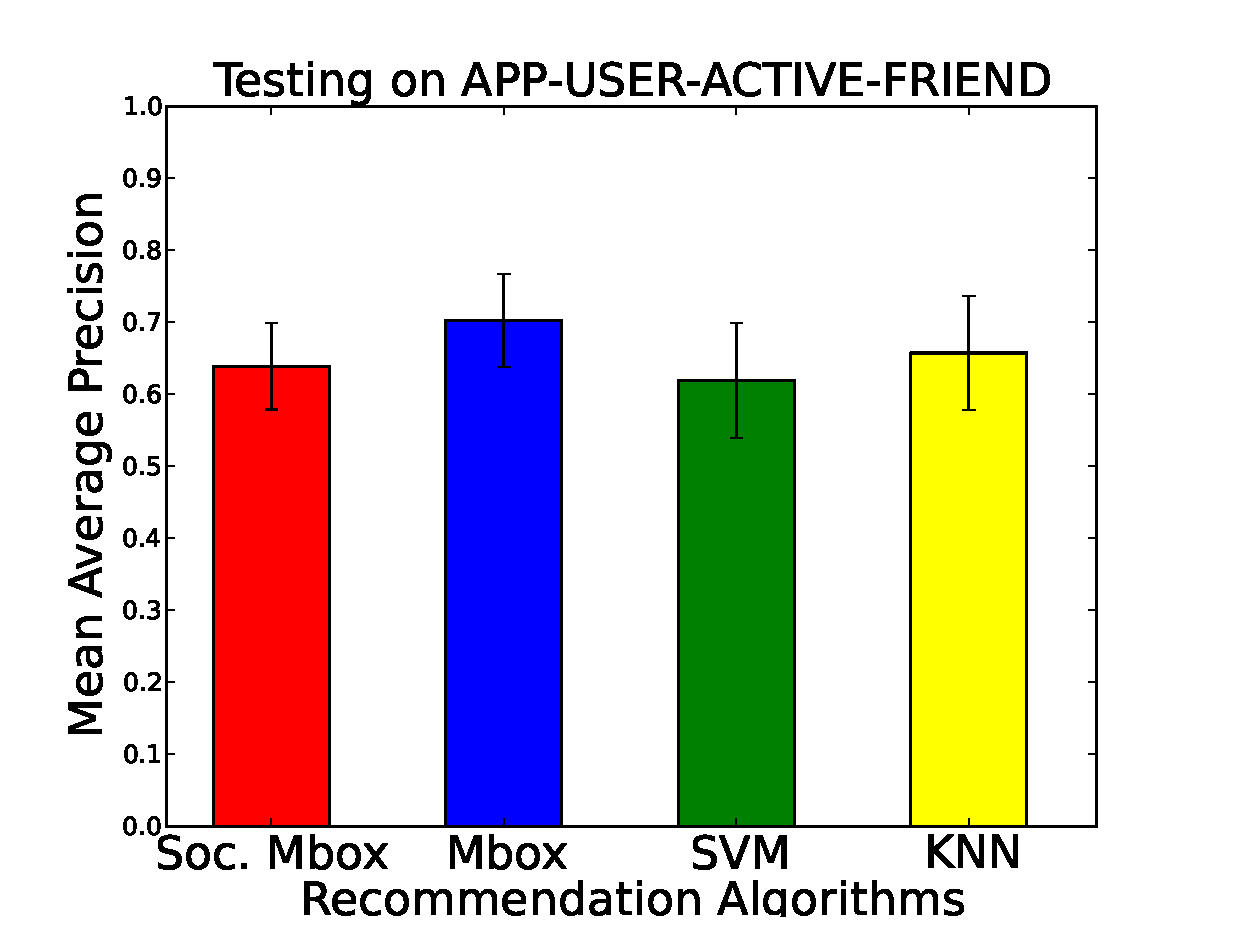
\includegraphics[scale=0.35]{img/Union_App-User-Active-Friends1.eps}}
\subfigure{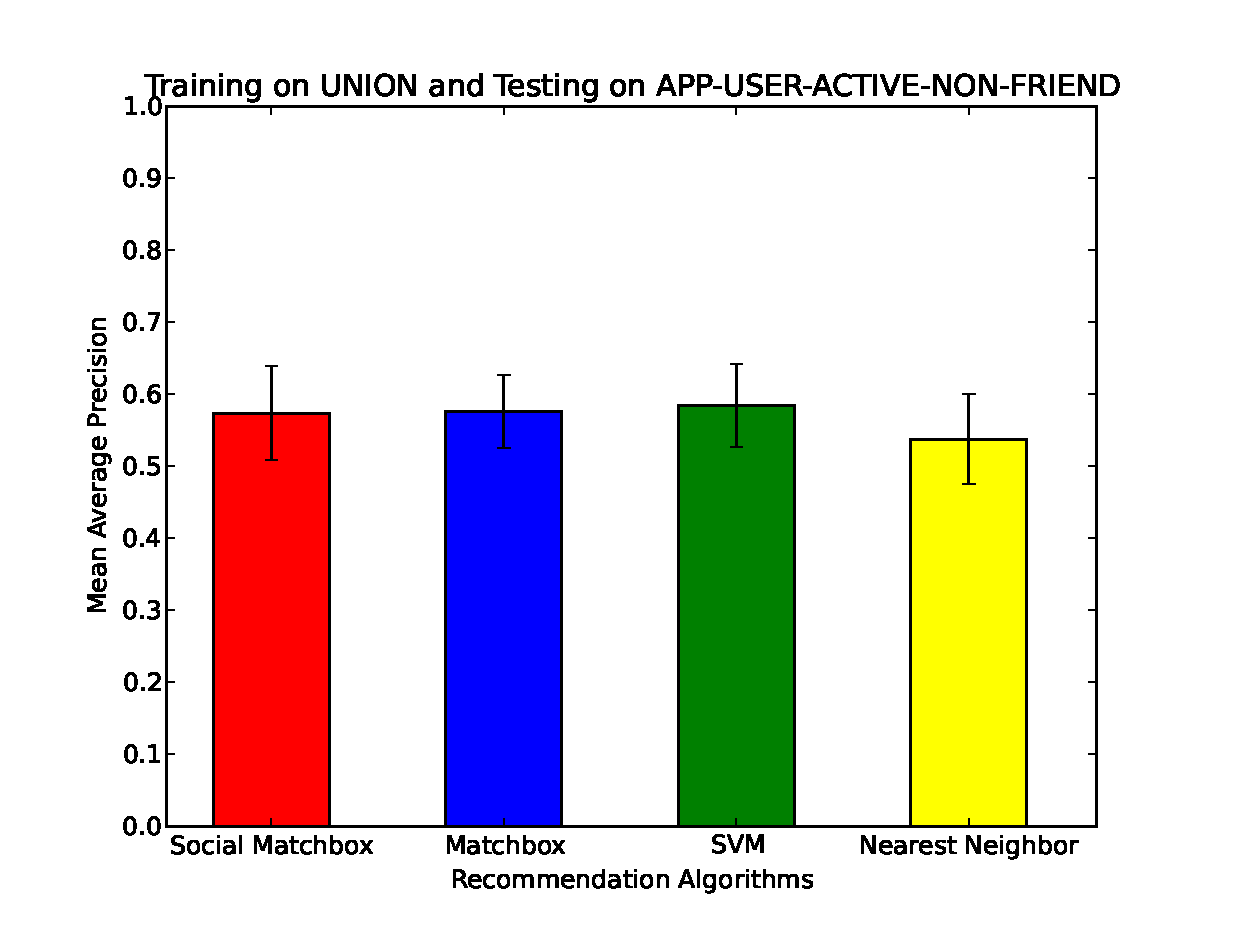
\includegraphics[scale=0.35]{img/Union_App-User-Active-NonFriends1.eps}}
\caption{Results of training on UNION data. When testing on APP-USER-ACTIVE-ALL, we find that Social Matchbox was again the best recommendation algorithm. Training on UNION and testing on APP-USER-ACTIVE-ALL is the training/test data combination that is most similar to the online setup.}
\end{figure}

\section{Survey Results}

Near the end of the first trial, the LinkR users were invited to answer a survey regarding their experiences with the recommendations they were getting. They were asked a number of questions, with the following pertaining to the quality of the recommendations:

\begin{itemize}
\item{Do you find that ANU LinkR recommends interesting links that you may not have otherwise seen?}
\item{Do you feel that ANU LinkR has adapted to your preferences since you first started using it?}
\item{How relevant are the daily recommended links?}
\item{Overall, how satisfied are you with LinkR?}
\end{itemize}

They gave their answers to each question as an integer rating with range $[1-5]$, with a higher value being better. Their answers were grouped together according to the recommendation algorithm that was assigned to them, and the averages per algorithm are below.

As shown in Figure~\ref{fig:survey1}, we see that Social Matchbox achieved higher scores than the other recommendation algorithms, in all four questions. The results of the survey reflected the results in the online live trial and confirms that Social Matchbox was the best recommendation algorithm in the first trial.
 
\begin{figure}[h]
\centering
\subfigure{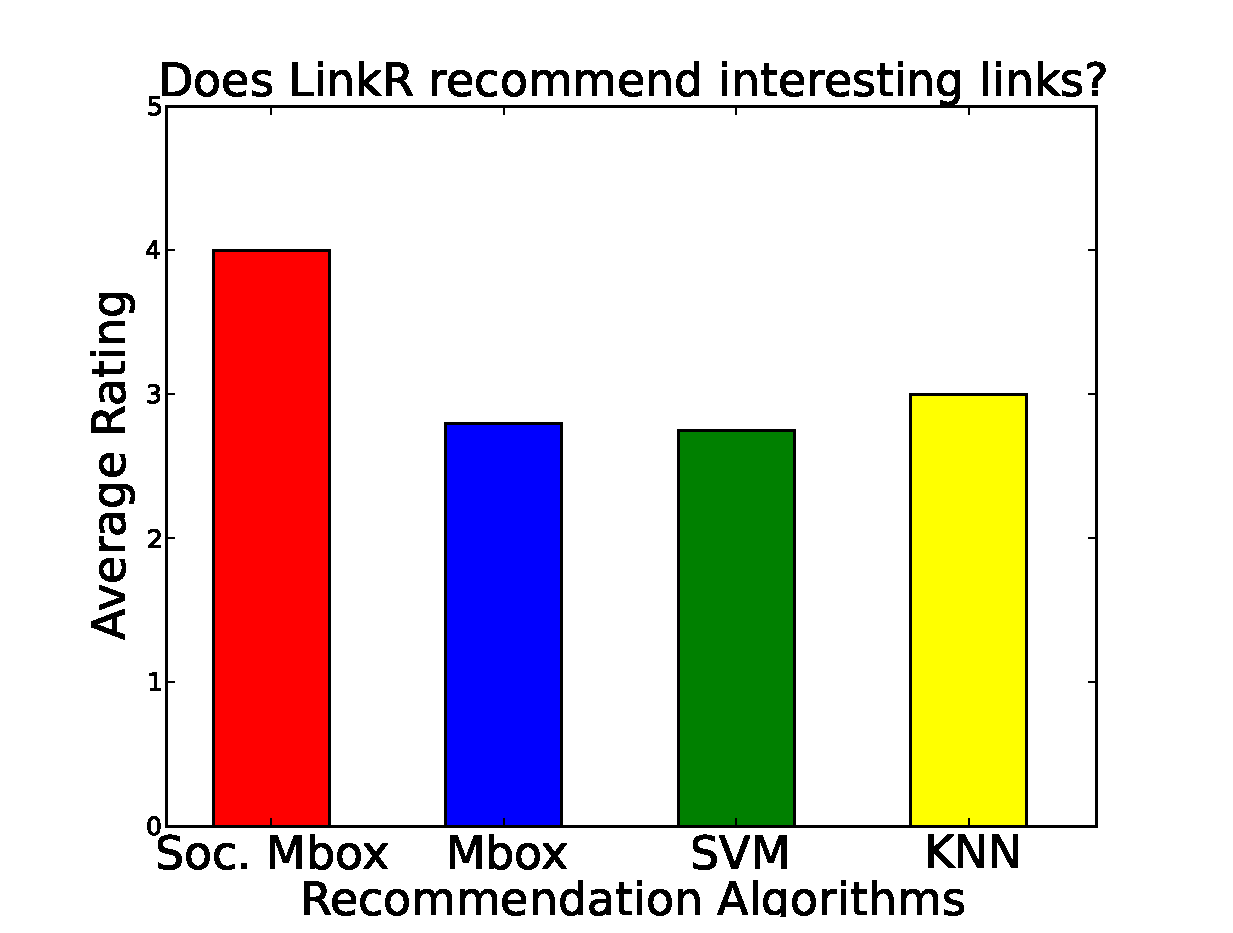
\includegraphics[scale=0.35]{img/not-seen.eps}}
\subfigure{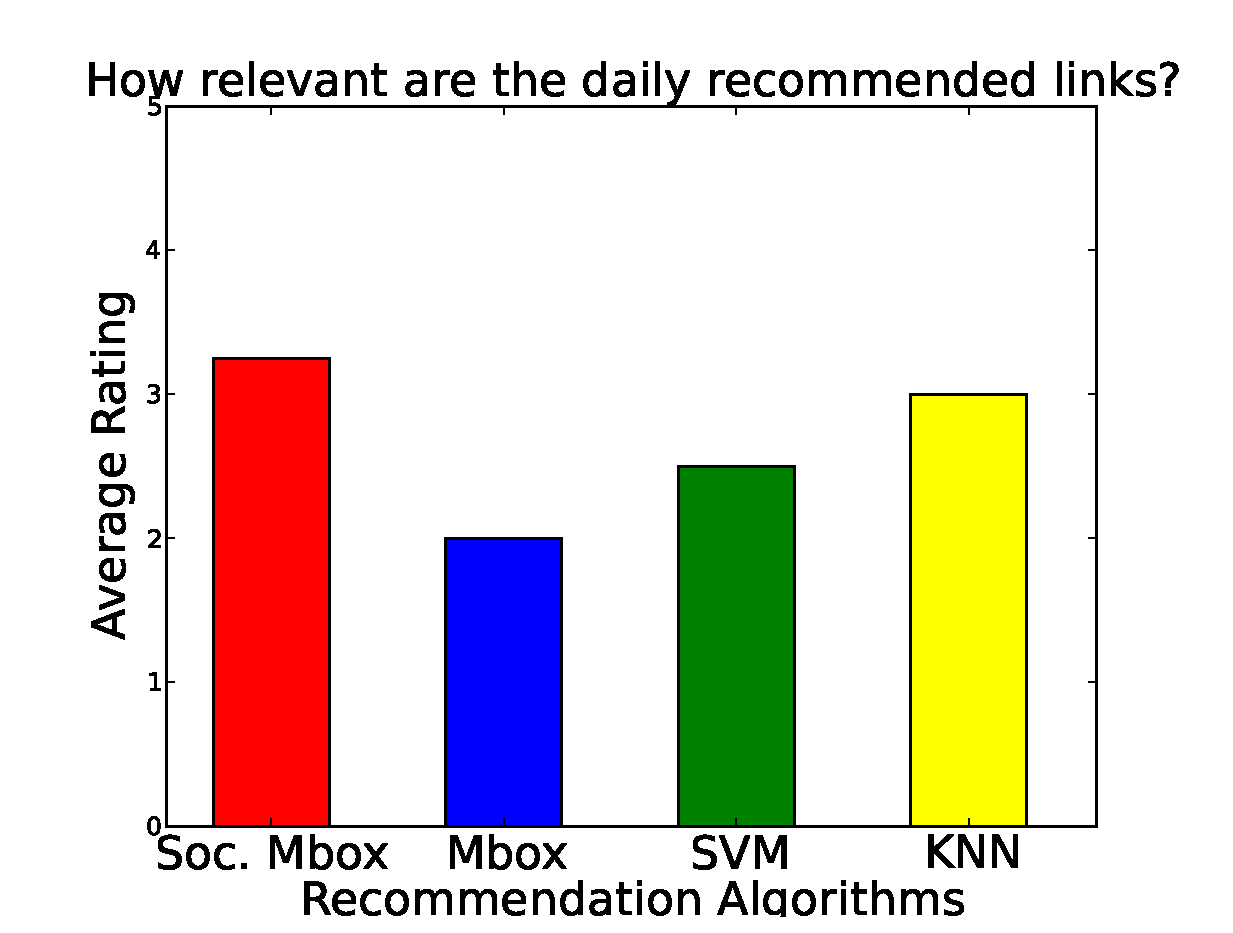
\includegraphics[scale=0.35]{img/relevant.eps}}
\subfigure{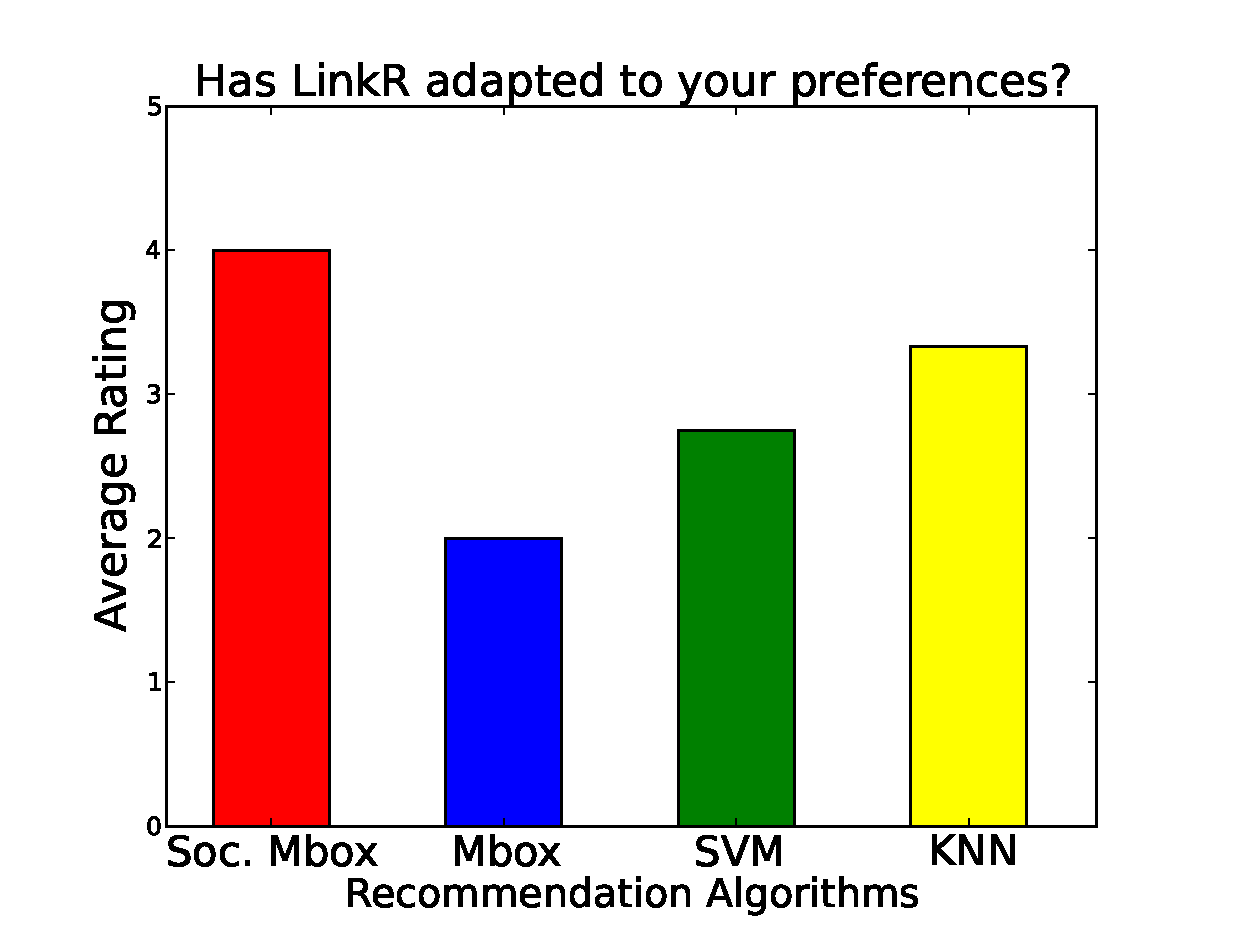
\includegraphics[scale=0.35]{img/adapted.eps}}
\subfigure{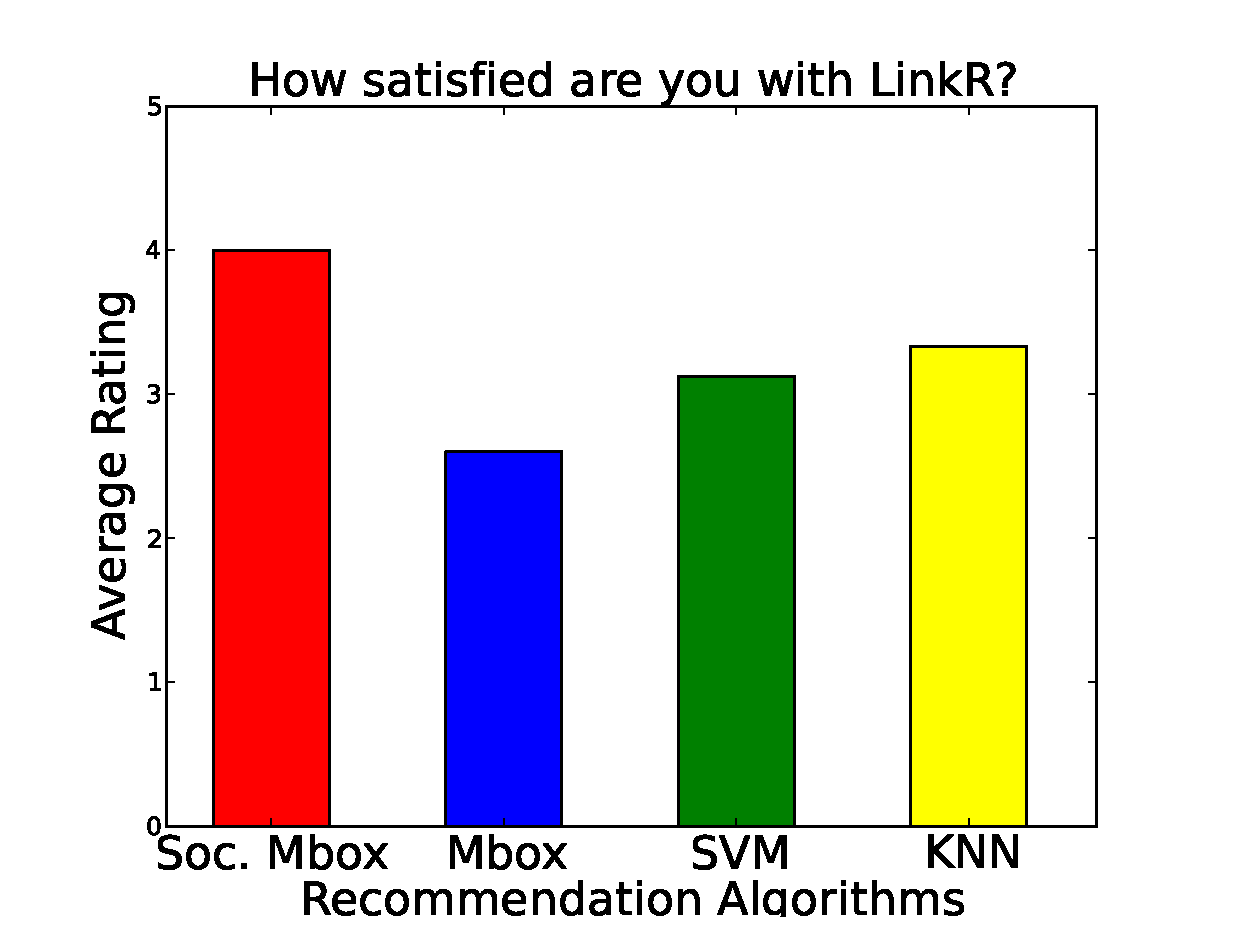
\includegraphics[scale=0.35]{img/satisfied.eps}}
\caption{Results of the user survey after the first trial. The survey answers from the users reflect the online results that Social Matchbox was the best recommendation algorithm in this trial.}
\label{fig:survey1}
\end{figure}

At the end of the first trial, we have seen that the Social Matchbox with its Social Regularization method does indeed outperform existing collaborative filtering recommenders. In the next chapter, we discuss new techniques for incorporating social information and show how they improve on Social Matchbox.
